\chapter{Analýza}

Pro vývoj aplikace v této bakalářské práci byla zvolena novější - agilní - metodika vývoje, která je v mnoha ohledech jednodušší než dříve používaný Rational Unified Process (RUP)\cite{rup}. Hlavní výhoda spočívá v tom, že se nevytváří velké množství dokumentů, jejichž vytvoření zabere mnoho času a většina z nichž je ve finále zbytečná. RUP má smysl spíše u~velkých projektů, na kterých pracuje větší tým lidí a které jsou hodně rozsáhlé. 

RUP a agilní metodiky se liší už ve způsobu sběru požadavků. Zatímco RUP je orientovaný na use-case modely, vytvářené obvykle v jazyce Unified Modeling Language (UML)\cite{uml}, agilní metodiky evidují požadavky v podobě tzv. user stories \cite{userstory}.

\section{User stories}

Požadavky v rámci agilních metodik se nezapisují jako prosté úkoly, ale mají formát tzv. user story. Jejich tvar je pevně daný a skládá se ze tří částí:
\begin{quote}
Jako \textbf{Uživatel}, chci \textbf{Funkcionalitu}, abych dostal \textbf{Bussiness Value}
\end{quote}

Takto formulovaný požadavek je pro člověka mnohem srozumitelnější, protože vidí, proč daný úkol splnit a jaký je jeho přínos. Má tak jistotu, že nedělá něco zbytečného. User story je takový krátký příběh a jako takový je lidským mozkem snáz vnímatelný.

User stories poslouží i po ukončení vývoje - při akceptačních testech. Stačí projít seznam user stories, a pokud je v aplikaci nalezen jejich \uv{odraz}, test byl úspěšný. Proto je lepší, aby user stories prošly schválením od zadavatele ještě před začátkem vývoje aplikace.

V rámci této bakalářské práce byl vytvořen následující seznam user stories, který je pro lepší přehlednost rozdělen do bloků podle cílové skupiny. Každý blok je uveden názvem role, kde lomítko značí \uv{dědičnost}. Jsou v něm zachyceny všechny požadavky, které by měla aplikace po ukončení vývoje splňovat.

\subsection{Uživatel}

Jako uživatel chci:

\begin{itemize}
\item používat aplikaci co nejjednodušeji, abych se mohl plně soustředit na přesné zadání úkolu
\item vytvářet úkoly, abych na nic nezapomněl
\item vytvářet projekty, abych si mohl úkoly třídit
\item vkládat okamžité nápady do inboxu s tím, že je později zatřídím do projektu
\item označit úkol jako splněný
\item uložit úkol do archivu pro případ, že bych se k němu chtěl někdy později vrátit
\item vyhodit úkol do koše, pokud se rozhodnu, že ho nebudu realizovat
\item přiřazovat úkolům štítky, abych si mohl odfiltrovat úkoly z určité oblasti
\item na konci týdne vědět, co všechno jsem za týden stihl, abych si mohl lépe naplánovat úkoly na příští týden
\item své nápady, na které teď nemám čas, přiřadit do skupiny s delším časovým horizontem, abych na ně nezapomněl a mohl je později rozvíjet
\item vytisknout svoje úkoly, abych je mohl mít neustále na očích
\end{itemize}

\subsection{Uživatel \slash  vývojář}

Jako vývojář chci:

\begin{itemize}
\item importovat projekty a úkoly z verzovacích serverů
\item být informován o blížící se deadline úkolů
\item aby aplikace neumožňovala přístup neoprávněným osobám k mým úkolům
\item spárovat úkol s konkrétním commitem do repozitáře
\item exportovat úkol a poslat ho jednoduše kolegovi v týmu, aby ho nemusel ručně přepisovat
\end{itemize}

\subsection{Uživatel \slash  vývojář \slash  senior}

Jako senior vývojář chci: 

\begin{itemize}
\item párovat repozitáře z verzovacích serverů s mými projekty, abych mohl sledovat, jak práce na projektu pokračuje
\item párovat issues ze serveru s mými úkoly, abych s nimi mohl párovat commity
\item nastavit úkolům čas, kdy mají být splněny
\item delegovat úkoly junior vývojářům
\item přiřadit úkol do konkrétního milníku, abych měl přehled o tom, kolik toho ještě zbývá dokončit
\item být informován o změnách v mých repozitářích na serverech
\item uzavřít projekt po jeho dokončení příp. předčasném ukončení
\item přiřazovat štítky k úkolům, abych je mohl lépe třídit a filtrovat
\item být upozorněn na neaktivní otevřené projekty, abych mohl urgovat dokončení úkolů na junior vývojářích
\item mazat úkoly, které se nakonec realizovat nebudou
\item zpřesňovat zadání úkolů, pokud dojde k nejasnostem
\end{itemize}

\subsection{Uživatel \slash  vývojář \slash  junior}

Jako junior vývojář chci:

\begin{itemize}
\item být informován o nově přiřazených úkolech od senior vývojářů
\item označit úkol jako splněný
\end{itemize}

\section{Doménový model}
Z výše zmíněných user stories byl v dalším kroku vytvořen seznam entit, které byly logicky provázány asociacemi. Pro lepší znázornění těchto entit a vztahů mezi nimi byl vytvořen doménový model v jazyce UML.

\begin{figure}[h]
	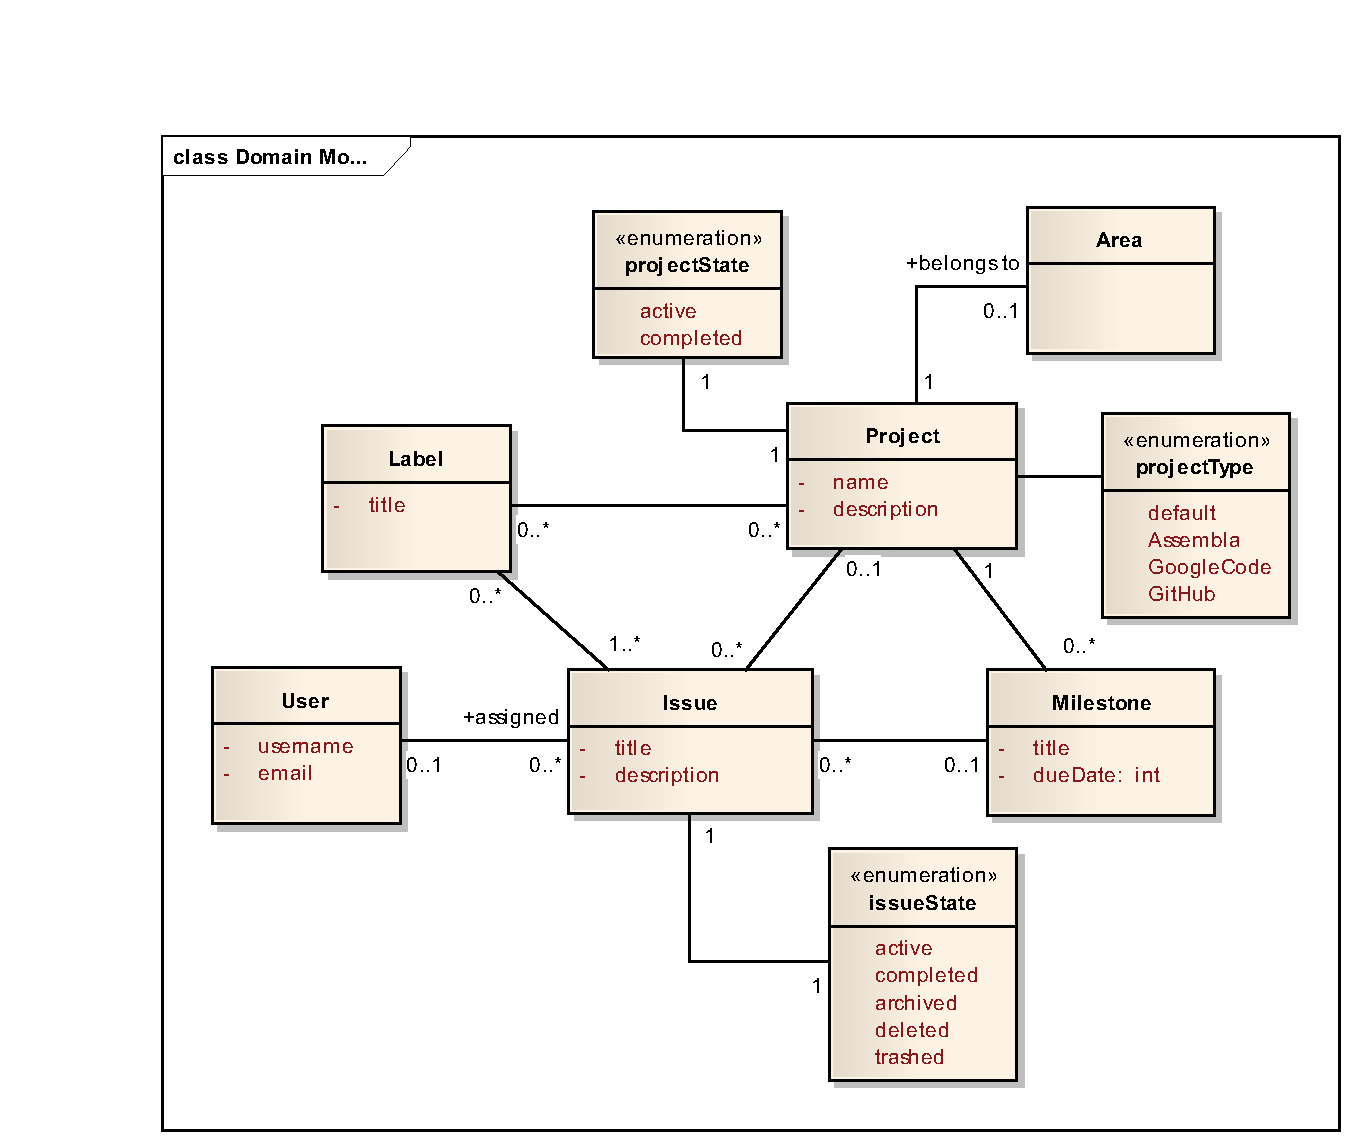
\includegraphics[keepaspectratio,width=16cm]{figures/domain-model}
	\caption{Doménový model}
	\label{fig:domain-model}
\end{figure}

\subsection{Issue}
Entita reprezentující jeden úkol, uložený v aplikaci. Má definované jméno (název problému) a popis, který obsahuje konkrétní charakteristiku problému

\subsection{IssueState}
Úkoly (issues) existují v aplikaci v různých stavech. Každý stav určuje, jak bude aplikace s daným úkolem zacházet \ref{tab:issueState}.

\begin{table}[h]
\begin{center}
	\begin{tabular}{|c|l|}
	\hline
	Atributy & Poznámky \\
	\hline
	active & na úkolu se pracuje \\
	completed & úkol byl splněn \\
	archived & úkol byl uložen do archivu \\
	deleted & úkol byl smazán \\
	trashed & úkol byl přesunout do koše \\
	\hline
	\end{tabular}
\end{center}
\caption{Vlastnosti entity IssueState}
\label{tab:issueState}
\end{table}

\subsection{Label}
Štítky (label) slouží k filtraci úkolů (issues) a projektů (projects). Obvykle popisují nějakou obecnější vlastnost dané entity, podle které má smysl je filtrovat. To může být například priorita, programovací jazyk nebo náročnost \ref{tab:label}.

\begin{table}[h]
\begin{center}
	\begin{tabular}{|c|l|}
	\hline
	Atributy & Poznámky \\
	\hline
	title & text štítku \\
	\hline
	\end{tabular}
\end{center}
\caption{Vlastnosti entity Label}
\label{tab:label}
\end{table}

\subsection{Milestone}
Milestone se do češtiny překládá jako milník. Je to nějaký bod v čase, do kterého musí být dokončena určitá množina úkolů (issues). Lze sledovat procentuální dokončení \ref{tab:milestone}.

\begin{table}[h]
\begin{center}
	\begin{tabular}{|c|l|}
	\hline
	Atributy & Poznámky \\
	\hline
	title & název milníku \\
	dueDate & do kdy musí být milník splněn \\
	\hline
	\end{tabular}
\end{center}
\caption{Vlastnosti entity Milestone}
\label{tab:milestone}
\end{table}

\subsection{User}
Uživatel (User) vystupuje v aplikaci jako člen týmu, kterému je možné přiřadit nějaký úkol (Issue) \ref{tab:user}.

\begin{table}[h]
\begin{center}
	\begin{tabular}{|c|l|}
	\hline
	Atributy & Poznámky \\
	\hline
	username & uživatelské jméno \\
	email & e-mailová adresa uživatele \\
	\hline
	\end{tabular}
\end{center}
\caption{Vlastnosti entity User}
\label{tab:user}
\end{table}

\subsection{Project}
Úkoly (issues) jsou uspořádané do projektů, které mají definované jméno a popis. I z úkolu se může stát projekt, pokud je k jeho dokončení potřeba víc než jeden krok (podle GTD) \ref{tab:project}.

\begin{table}[h]
\begin{center}
	\begin{tabular}{|c|l|}
	\hline
	Atributy & Poznámky \\
	\hline
	name & název projektu \\
	description & popis projektu \\
	\hline
	\end{tabular}
\end{center}
\caption{Vlastnosti entity Project}
\label{tab:project}
\end{table}

\subsection{ProjectState}
Projekt může být buď aktivní, tzn. že se na něm pracuje, nebo dokončený \ref{tab:projectState}.

\begin{table}[h]
\begin{center}
	\begin{tabular}{|c|l|}
	\hline
	Atributy & Poznámky \\
	\hline
	active & aktivní \\
	completed & dokončený \\
	\hline
	\end{tabular}
\end{center}
\caption{Vlastnosti entity ProjectState}
\label{tab:projectState}
\end{table}

\subsection{ProjectType}

Každý projekt má definovaný nějaký typ, podle kterého se určí, na jaký server se má synchronizovat. Pokud jde o obyčejný projekt (default), nesynchronizuje se nikam, všechny úkoly zůstávají pouze na lokálním úložišti \ref{tab:projectType}.

\begin{table}[h]
\begin{center}
	\begin{tabular}{|c|l|}
	\hline
	Atributy & Poznámky \\
	\hline
	default & obyčejný GTD projekt \\
	Assembla & projekt hostovaný na serveru Assembla.com \\
	GoogleCode & projekt hostovaný na serveru Google Code \\
	GitHub & projekt hostovaný na serveru GitHub.com \\
	\hline
	\end{tabular}
\end{center}
\caption{Vlastnosti entity ProjectType}
\label{tab:projectType}
\end{table}

\subsection{Area}

Projekty (project) lze zařadit do nějaké oblasti (area), což může být např. škola, práce, vzdělávání apod. Cílem je zpřehlednění seznamu projektů.